\subsection{Dataset Preparation}
The dataset that we used in training basic Seq2Seq model is Cornell Movie-Dialogs Corpus \cite{corpus}, which comprises of 220,579 conversational exchanges extracted from raw movie scripts on IMDB, between 10,292 pairs of movie characters from 617 movies. 

Depends on whether the context is considered or not during the training, the dataset is treated differently For different models. For training the original seq2seq model, if a response has more than one line of sentence, we only take the first one. For example:

\begin{itemize}
\item[~] \textbf{Cameron}: \textit{Gigglepuss is playing there tomorrow night.}
\item[~] \textbf{Patrick}: \textit{So what does that give me?  I'm supposed to buy her some noodles and a book and sit around listening to chicks who can't play their instruments?}
\end{itemize}

becomes

\begin{itemize}
\item[~] \textbf{Cameron}: \textit{Gigglepuss is playing there tomorrow night.}
\item[~] \textbf{Patrick}: \textit{So what does that give me?}
\end{itemize}

On the other hand, for training VNRAE model we introduce the concept of sliding window as representation of context.


In addition, in order to fit the training tensor, we also set the limit to maximum length of each input line. The sentence length limit


Each word in a sentence is tokenized and added to the vocabulary. The total vocabulary size of the Cornell Movie-Dialogs Corpus adds up to 35,147 different words, which are used to build look-up table later in the training phase.

\subsection{Training environment}
We use 300 hidden units for each LSTM, along with the learning rate $\eta=0.001$ and momentum $\gamma=0.9$ as the hyper parameters. The training takes place in Amazon AWS EC2 instance p2.xlarge, with single NVIDIA Tesla K80 GPU and CUDA accerlation. Consider the long training time (around 4 hours per epoch if we use all the data), we decide not to sacrafice any data but reduce the number of epochs for this midway report, since a trained model can always be fine-tuned with additional epochs in the future. For the current stage, we reached a model with a 10 epochs, which seems to still have some basic chatting ability (see below).

\subsection{Various Context Sizes of Conversation}


\subsection{Results and discussion}

As shown in the figure \ref{fig:loss}, we are pretty sure that the we haven't reach the minimum of our LSTM loss function at current stage. The model still have leeway for improvement in the future given enough additional epochs.

\begin{figure}[H]
\centering
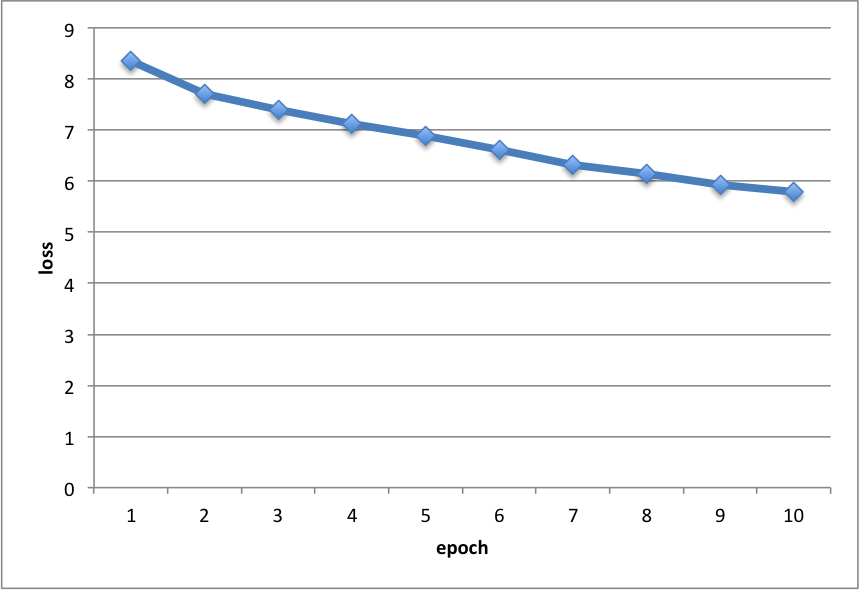
\includegraphics[width=0.4\textwidth]{loss.png}
\caption{Training of a basic Seq2Seq model}
\label{fig:loss}
\end{figure}

To demonstrate the result, here we provide a sample of conversation:

\begin{itemize}
\item[~] \textbf{Input}: \textit{Hi.}
\item[~] \textbf{Bot}: \textit{Hi.}
\item[~] \textbf{Input}: \textit{How are you?}
\item[~] \textbf{Bot}: \textit{I don't know.}
\item[~] \textbf{Input}: \textit{Why?}
\item[~] \textbf{Bot}: \textit{Because i'm a little confused.}
\item[~] \textbf{Input}: \textit{Are you a machine?}
\item[~] \textbf{Bot}: \textit{I'm not.}
\item[~] \textbf{Input}: \textit{Are you sure?}
\item[~] \textbf{Bot}: \textit{Yes.}
\item[~] \textbf{Input}: \textit{What's your name?}
\item[~] \textbf{Bot}: \textit{I'm not going to let you get away with it.}
\item[~] \textbf{Input}: \textit{You are kidding...right?}
\item[~] \textbf{Bot}: \textit{No.}
\end{itemize}

At first, the response form our vanilla Seq2Seq seems reasonable, but there are still problems. First, the model gives a weird response after we input "What's your name?" This is probably because our model doesn't reach the optimum. Second, the constrain of this model doesn't have generative ability. After few tests, we can observe that the model will always give the same response for a given input. Lastly, the Seq2Seq model only consider the short-term memory inside each sentence pairs but the long-term memory in the history of conversation. In other words, if we ask "Are you sure?", the current model will always answer "Yes" regardless the previous question. Therefore, in the future we want to see if incoporating VAE with Seq2Seq can solve these problems and improve the chatting performance.

\subsection{Incoming experiments for combining}
\subsubsection{Data and prepossessing}
For our experiments, the raw dataset including original subtitles from movies. In order to feed our data into model, we need to perform some prepossessing. We will split the sequence of communication into pair of dialogues using the information of time intervals between sentences. More specifically, if the difference of time labels for two neighborhood sentences are within several seconds, then they can form a pair of dialogue, which means the last sentence can be seen as a response to first sentence. Moreover, we will only take the first line of sentences if there are multiple lines within the last sentences. After we construct pairs of sentences, we will perform word embedding in order to turn terms in sentences into representative vectors. These vectors will be the input for our vanilla seq2seq model as well as variational recurrent auto-encoder.

\subsubsection{Training VRAE to combine with Seq2seq model}
The experiment is composed of two phases.

In the first stage, we train a VRAE with 300 hidden units on the dataset described in the last section. The dimensionality of latent spaces is to be tuned based on preliminary experiment. We will try a two dimensional latent space first for the convenience of visualization of latent units as well as saving training time. Since the optimizer is very important to the training of VRAE. We will tune the parameter of optimizer based on the lower bound of log likelihood and choose a reasonable parameter for our next experiments. If the parameter is fine tuned, we should see that the location of data points in the two-dimensional latent space distributed according some patterns instead of just randomly distributed. However, a simple two dimensional latent space may not be able to fully capture the information of dialogues. Thus, we will perform VRAE with higher dimensional multivariate Gaussian latent variables. Note that as the number of dimensions increase, we will need more training time for VRAE. Here, the capacity of model and the computing resources are a trade-off that we need to balance.

For the first stage, we will get the change of lower bound versus epochs, latent variables vector and corresponding samples draw from the latent variables for two dimensional latent space as well as a higher dimensional latent space.

In the second stage, we append the sampling vectors as context information to the dense vector of Seq2seq model. We will make a comparison between the vanilla Seq2seq model and the improved one with context information appended. Then we will test the quality of generated dialogue with quantitative BLEU score as well as qualitative human judgements.